\documentclass{article}

\usepackage{arxiv}

\usepackage[utf8]{inputenc} % allow utf-8 input
\usepackage[T1]{fontenc}    % use 8-bit T1 fonts
\usepackage{hyperref}       % hyperlinks
\usepackage{url}            % simple URL typesetting
\usepackage{booktabs}       % professional-quality tables
\usepackage{amsfonts}       % blackboard math symbols
\usepackage{nicefrac}       % compact symbols for 1/2, etc.
\usepackage{microtype}      % microtypography
\usepackage{cleveref}       % smart cross-referencing
\usepackage{lipsum}         % Can be removed after putting your text content
\usepackage{graphicx}
\usepackage{natbib}
\usepackage{doi}
\usepackage{caption}
\usepackage{subcaption}

\def\tightlist{}

\title{Compositional Metabolic Flux Analysis}

\date{}

\usepackage{authblk}
\renewcommand\Authfont{\bfseries}
\setlength{\affilsep}{0em}
\newbox{\orcid}\sbox{\orcid}{
\includegraphics[scale=0.06]{orcid.pdf}} 


\author[1]{
  \href{asdfasdef}{\usebox{\orcid}\hspace{1mm}Teddy Groves}
}
\author[1]{
  \href{asdfasdef}{\usebox{\orcid}\hspace{1mm}Te Chen}
}
\author[1]{
  \href{asdfasdef}{\usebox{\orcid}\hspace{1mm}Sergi Muyo Abad}
}
\author[1]{
  \href{asdfasdef}{\usebox{\orcid}\hspace{1mm}Nicholas Luke Cowie}
}
\author[1]{
  \href{asdfasdef}{\usebox{\orcid}\hspace{1mm}Daria Volkova}
}
\author[2]{
  \href{asdfasdef}{\usebox{\orcid}\hspace{1mm}Christian Brinch}
}
\author[1,3]{
  \href{asdfasdef}{\usebox{\orcid}\hspace{1mm}Lars Keld Nielsen}
}

\affil[1]{The Novo Nordisk Center for Biosustainability, DTU, Kongens
Lyngby, Denmark}
\affil[2]{National Food Institute, DTU, Kongens Lyngby, Denmark}
\affil[3]{Australian Institute for Bioengineering and Nanotechnology
(AIBN), The University of Queensland, St Lucia 4067, Australia}


% \renewenvironment{abstract}
%  {\small
%   \begin{center}
%   \bfseries \abstractname\vspace{-.5em}\vspace{0pt}
%   \end{center}
%   \list{}{
%     \setlength{\leftmargin}{1.5cm}%
%     \setlength{\rightmargin}{\leftmargin}%
%   }%
%   \item\relax}
% {\endlist}

\hypersetup{
	pdftitle={Compositional Metabolic Flux Analysis},
	pdfauthor={ Teddy Groves,   Te Chen,   Sergi Muyo Abad,   Nicholas Luke
Cowie,   Daria Volkova,   Christian Brinch,   Lars Keld Nielsen,   },
    colorlinks=true,
    linkcolor=black,
    filecolor=black,
    urlcolor=black,
	citecolor=black
}
\begin{document}
\maketitle

\begin{abstract}
	Metabolic Flux Analysis aims to infer the values of metabolic fluxes
from measurements of isotope labelling distributions. Since these
distributions are positive, sum-constrained and relatively
low-dimensional, we argue that they should be analysed using specialised
methods that target compositional data. We illustrate our argument using
a simple pedagogical example, then show how compositional analysis leads
to improved results on a typical dataset.
\end{abstract}



\section{Note to Christian}\label{note-to-christian}

Metabolism refers to all chemical reactions that occur within living
cells, allowing organisms to grow, reproduce, and respond to their
environment. These reactions form interconnected networks called
metabolic pathways, where each step converts one molecule to another
through enzymatic reactions. Just as understanding traffic flow in a
city requires knowing not just the road layout but also how many
vehicles travel each route, understanding cellular function requires
knowing both the structure of metabolic pathways and the rates at which
molecules flow through them. These rates are called ``metabolic
fluxes.'' While measuring the concentrations of molecules (metabolites)
in a cell is relatively straightforward with modern techniques,
determining how quickly these molecules are being produced, converted,
or consumed inside the cell remains challenging. Scientists have
developed approaches using isotopes---variants of elements with
different atomic weights---as tracers to track the flow of atoms through
metabolic pathways. These isotopes act like molecular GPS trackers,
allowing researchers to follow the journey of specific atoms through the
complex network of cellular metabolism. The following section explains
how these isotope-based approaches work and introduces a new perspective
on analyzing the resulting data.

\section{Introduction}\label{introduction}

The rates, or ``fluxes'', of metabolic reactions are key to
understanding how cells behave. The rates of internal metabolic
reactions, which create and destroy chemicals inside of cells, are
particularly interesting, but difficult to measure directly. Isotope
labelling experiments make it possible to infer these internal fluxes
indirectly, thanks to the fact that metabolic reactions split and join
molecules in predictable ways.

Specifically, given a known ``atom mapping'' describing how each
reaction in a network moves potentially-labelled atoms, a specification
of fluxes, and some known isotope distributions (typically the feed),
one can calculate expected isotope distributions for internal
metabolites. These internal isotope distributions can also be measured,
for example using liquid chromatography and mass spectrometry. Comparing
measured and expected isotope distributions makes it possible to say
infer flux specifications.

This technique has existed in its modern form for a while, leading to
impressive results, but we think that a crucial step is missing.
Measured and expected isotope distributions are compositions, but they
have not previously been analysed using compositional methods.

\subsection{Isotopes, isotopomers and
isotopologues}\label{isotopes-isotopomers-and-isotopologues}

Isotopes are atoms whose nuclei have the same number of protons but
different numbers of neutrons. Isotopes of the same element have similar
chemical properties, but have different atomic masses and physical
properties. For example, carbon has three naturally occurring isotopes:
12C, 13C and 14C, with respective atomic masses 12, 13 and 14. 14C
occurs in negligible quantities, and the natural ratio of 12C to 13C is
known, making carbon suitable for isotope labelling experiments where
12C is artificially replaced by 13C.

Isotopomers are forms of a compound that differ only by substitution of
isotopes. For example, {[}1-13C{]} glucose and {[}2-13C{]} glucose are
isotopomers of glucose that differ only in the isotopes of the carbon
atoms in positions 1 and 2 (see \hyperref[glucose]{figure below}). In
general, for every \(a\) occurrences of an atom with \(I\) isotopes in a
compound, there are \(I^a\) corresponding isotopomers. For example,
glucose has six carbon atoms: assuming only 12C and 13C isotopes are
present, there are \(2^6=64\) carbon isotopomers.

\begin{figure}[!h]
\centering
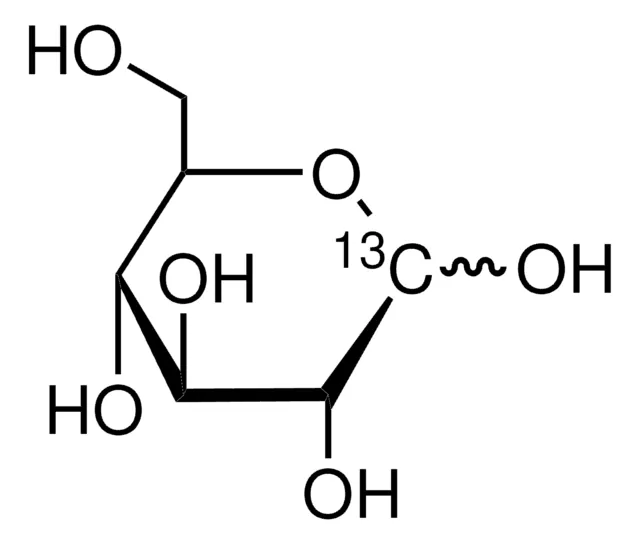
\includegraphics[width=0.4\textwidth, height=!]{img/1-13C-glucose.png}
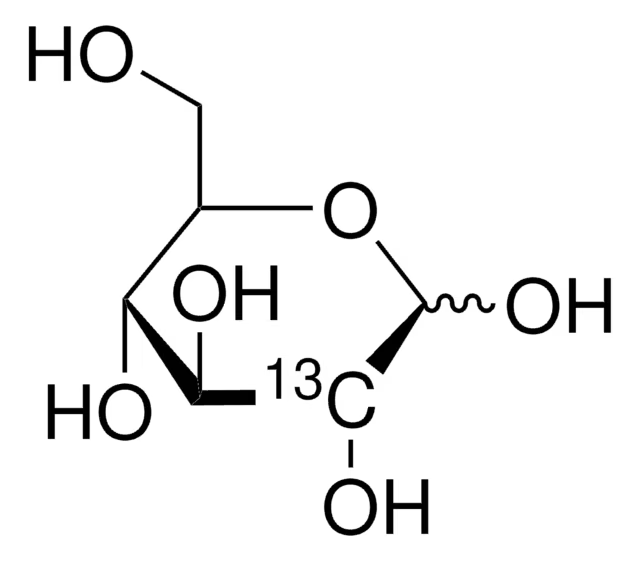
\includegraphics[width=0.4\textwidth, height=!]{img/2-13C-glucose.png}
\caption{Left: [1-13C] glucose Right: [2-13C] glucose}
\label{glucose}
\end{figure}

Isotopologues are forms of a compound that differ in atomic mass. For
example, the isotopomers {[}1-13C{]} glucose and {[}2-13C{]} glucose
each have five 12C atoms and one 13C atom and therefore belong to the
same isotopologue \(M_1\) with atomic mass 181.15 g/mol. Isotopologues
are important because measurements can often distinguish between
isotopologues, but not between isotopomers with the same atomic mass.

\subsection{Isotope labelling based Metabolic Flux
Analysis}\label{isotope-labelling-based-metabolic-flux-analysis}

In more detail, MFA considers a known metabolic network consisting of
\(M\) compounds and \(N\) reactions with stoichiometric coefficients
\(S\in\mathbb{R}^{M\times N}\) representing the amount of each compound
consumed and produced by each reaction, plus an atom transition map for
each reaction. The atom transition map for a reaction specifies in what
order the potentially-labelled atoms occur in each of the reaction's
substrates and products.

In this study we focus on the most straightforward case, where it is
safe to assume that the network is in isotopic and metabolic steady
state. This means that the concentrations of internal metabolites and
isotopomers are constant.

The remaining input for MFA is as follows:

\begin{itemize}
\item
  Known isotopomer proportions for some compounds, typically external
  ones like the feed.
\item
  Measured fluxes for some reactions.
\item
  Measured isotopologue proportions for some compounds, possibly with
  known measurement error.
\end{itemize}

The ``forward problem'' of inferring the label pattern given a flux
specification can be solved by writing down a balance equation
describing the rate of change of each isotopomer in the network. These
equations can be found by combining the atom map and stoichiometric
matrix to produce a matrix \(S_i\in\mathbb{R}^{I\times N}\) of
stoichiometric coefficients for isotopomers. At isotopic and metabolic
steady state we have \(Sv=0\), giving \(N\) balance equations. Given
some known isotopomer proportions, other isotopomer proportions can be
calculated by solving these equations.

While conceptually simple, this approach to solving the forward problem
is typically unfeasible due to the prohibitively large number of
isotopomers. Practical applications therefore require a method to solve
the forward problem more simply: see
\citep[§3.1]{daiUnderstandingMetabolismFlux2017} for an overview of
approaches to this problem. The most widely used of these is the
``elementary metabolite unit'' representation introduced in
\citep{antoniewiczElementaryMetaboliteUnits2007}.

The inverse problem of inferring steady state fluxes from measured
isotopomer or isotopologue distributions can be solved using a
statistical model that links these measurements with latent parameters
representing flux configurations. In general, such a model specifies the
probability \(p(r_{obs}\mid r(v))\) of observing labelling pattern
\(r_{obs}\) given a true flux assignment \(v\) and true labelling
pattern \(r(v)\). For example, assuming an independent linear model with
measurement standard deviation vector \(\sigma\) yields the following
relationship:

\[
p(r_{obs}\mid r(v)) = pdf_{normal}(r_{obs} | r(v), \sigma)
\label{linear}
\]

Sometimes a statistical model is not mentioned explicitly, but \(v\) is
optimised by minimising a scaled Euclidean distance from \(r(v)\) to
\(r_{obs}\), which produces the same result as optimising by maximising
the likelihood \hyperref[linear]{\(p(r_{obs}\mid r(v))\)}.

\subsection{Previous work}\label{previous-work}

This section briefly reviews previous work in labelling-based metabolic
flux analysis. For more detailed review papers see
\citep{daiUnderstandingMetabolismFlux2017},
\citep{falcoMetabolicFluxAnalysis2022}.

\subsubsection{Experimental methods}\label{experimental-methods}

See the following references:

\begin{itemize}
\tightlist
\item
  \citep{longHighresolution13CMetabolic2019}
\item
  \citep{falcoMetabolicFluxAnalysis2022}
\end{itemize}

\subsubsection{Bayesian methods}\label{bayesian-methods}

See the following references:

\begin{itemize}
\tightlist
\item
  \citep{theorellBeCertainUncertainty2017}
\item
  \citep{theorellReversibleJumpMCMC2020}
\end{itemize}

\subsubsection{Software}\label{software}

Existing implementations of MFA include:

\begin{itemize}
\tightlist
\item
  INCA
\item
  13CFLUX2
\item
  Metran
\item
  OpenFlux(2)
\item
  FluxPyt
\item
  mfapy
\item
  Sysmetab
\item
  iso2flux
\item
  Flux-P
\item
  WUFlux
\item
  OpenMebius
\item
  influx\_s
\end{itemize}

See {[}REFERENCE{]} for reviews of available software implementing MFA.

There is no previous implementation of compositional regression analysis
in the context of MFA; all previous implementations apply a linear model
either explicitly as in \citep[Eq. 3]{theorellBeCertainUncertainty2017}
or more commonly implicitly through the use of Euclidean distance based
optimisation.

\section{Problem statement}\label{problem-statement}

Discrepancies between observed and expected isotopologue distributions
have previously been modelled using linear regression models, despite
the fact that both are compositions. It is well known that, in general,
applying non-compositional data analysis methods to compositional data
is dangerous because these methods can easily misinterpret
constraint-induced correlations \citep[Ch.
3]{aitchisonjStatisticalAnalysisCompositional}. This issue is especially
pronounced in the case where there are relatively few composition
components.

We therefore propose modelling augmenting existing labelling-based MFA
methods with specialised compositional data analysis. In this section we
draw on previous literature where compositional data analysis to discuss
common arguments against the use of specialised compositional methods,
explaining why we think they don't apply in the case of labelling based
MFA.

\subsection{Arguments against using compositional
methods}\label{arguments-against-using-compositional-methods}

\section{Simple pedagogical example}\label{simple-pedagogical-example}


\bibliographystyle{unsrtnat}
\bibliography{refs.bib}
\end{document}
